
% LaTeX Beamer file automatically generated from Doconce
% http://code.google.com/p/doconce

%-------------------- begin preamble ----------------------

\documentclass{beamer}

\usetheme{red3}
\usecolortheme{default}

% turn off the almost invisible, yet disturbing, navigation symbols:
\setbeamertemplate{navigation symbols}{}

% Examples on customization:
%\usecolortheme[named=RawSienna]{structure}
%\usetheme[height=7mm]{Rochester}
%\setbeamerfont{frametitle}{family=\rmfamily,shape=\itshape}
%\setbeamertemplate{items}[ball]
%\setbeamertemplate{blocks}[rounded][shadow=true]
%\useoutertheme{infolines}
%
%\usefonttheme{}
%\useinntertheme{}
%
%\setbeameroption{show notes}
%\setbeameroption{show notes on second screen=right}

% fine for B/W printing:
%\usecolortheme{seahorse}

\usepackage{pgf,pgfarrows,pgfnodes,pgfautomata,pgfheaps,pgfshade}
\usepackage{graphicx}
\usepackage{epsfig}
\usepackage{minted} % requires pygments and latex -shell-escape filename
\usepackage{fancyvrb,relsize}
\usepackage{amsmath,amssymb,bm}
%\usepackage[latin1]{inputenc}
\usepackage[utf8]{inputenc}
\usepackage{colortbl}
\usepackage[english]{babel}
\usepackage{tikz}
\usepackage{framed,anslistings}
% Use some nice templates
\beamertemplatetransparentcovereddynamic

% Delete this, if you do not want the table of contents to pop up at
% the beginning of each section:
\AtBeginSection[]
{
    \begin{frame}<beamer>[plain]
    \frametitle{}
    \tableofcontents[currentsection]
    \end{frame}
}

% Delete this, if you do not want the table of contents to pop up at
% the beginning of each section:
\AtBeginSection[]
{
    \begin{frame}<beamer>[plain]
    \frametitle{}
    \tableofcontents[currentsection]
    \end{frame}
}

% If you wish to uncover everything in a step-wise fashion, uncomment
% the following command:

%\beamerdefaultoverlayspecification{<+->}

\newcommand{\shortinlinecomment}[3]{\note{\textbf{#1}: #2}}
\newcommand{\longinlinecomment}[3]{\shortinlinecomment{#1}{#2}{#3}}

\newenvironment{notice_colors1admon}[1][]{\begin{block}{#1}}{\end{block}}
\newenvironment{notice_colors2admon}[1][]{\begin{block}{#1}}{\end{block}}
\newenvironment{notice_graybox3admon}[1][]{\begin{block}{#1}}{\end{block}}
\newenvironment{notice_yellowboxadmon}[1][]{\begin{block}{#1}}{\end{block}}
\newenvironment{summary_colors1admon}[1][]{\begin{block}{#1}}{\end{block}}
\newenvironment{summary_colors2admon}[1][]{\begin{block}{#1}}{\end{block}}
\newenvironment{summary_graybox3admon}[1][]{\begin{block}{#1}}{\end{block}}
\newenvironment{summary_yellowboxadmon}[1][]{\begin{block}{#1}}{\end{block}}
\newenvironment{warning_colors1admon}[1][]{\begin{block}{#1}}{\end{block}}
\newenvironment{warning_colors2admon}[1][]{\begin{block}{#1}}{\end{block}}
\newenvironment{warning_graybox3admon}[1][]{\begin{block}{#1}}{\end{block}}
\newenvironment{warning_yellowboxadmon}[1][]{\begin{block}{#1}}{\end{block}}
\newenvironment{question_colors1admon}[1][]{\begin{block}{#1}}{\end{block}}
\newenvironment{question_colors2admon}[1][]{\begin{block}{#1}}{\end{block}}
\newenvironment{question_graybox3admon}[1][]{\begin{block}{#1}}{\end{block}}
\newenvironment{question_yellowboxadmon}[1][]{\begin{block}{#1}}{\end{block}}
\newenvironment{block_colors1admon}[1][]{\begin{block}{#1}}{\end{block}}
\newenvironment{block_colors2admon}[1][]{\begin{block}{#1}}{\end{block}}
\newenvironment{block_graybox3admon}[1][]{\begin{block}{#1}}{\end{block}}
\newenvironment{block_yellowboxadmon}[1][]{\begin{block}{#1}}{\end{block}}
\newenvironment{paragraphadmon}[1][]{\begin{block}{#1}}{\end{block}}
\newenvironment{graybox1admon}[1][]{\begin{block}{#1}}{\end{block}}
\newenvironment{graybox2admon}[1][]{\begin{block}{#1}}{\end{block}}
\newcommand{\grayboxhrules}[1]{\begin{block}{}#1\end{block}}



% insert custom LaTeX commands...

\makeindex

%-------------------- end preamble ----------------------

\begin{document}


\renewcommand{\u}{\pmb{u}}

\newcommand{\xbm}{\bm{x}}
\newcommand{\normalvecbm}{\bm{n}}
\newcommand{\ubm}{\bm{u}}


\newcommand{\x}{\pmb{x}}
\newcommand{\normalvec}{\pmb{n}}
\newcommand{\Ddt}[1]{\frac{D#1}{dt}}
\newcommand{\halfi}{1/2}
\newcommand{\half}{\frac{1}{2}}
\newcommand{\report}{test report}


% ------------------- main content ----------------------



% ----------------- title -------------------------
\title{On Schemes for Exponential Decay}

% ----------------- author(s) -------------------------
\author{Hans Petter Langtangen\inst{1,2}}
\institute{Center for Biomedical Computing, Simula Research Laboratory\inst{1}
\and
Department of Informatics, University of Oslo\inst{2}}
% ----------------- end author(s) -------------------------


\date{Jun 29, 2013
\\ \ \\ 
\centerline{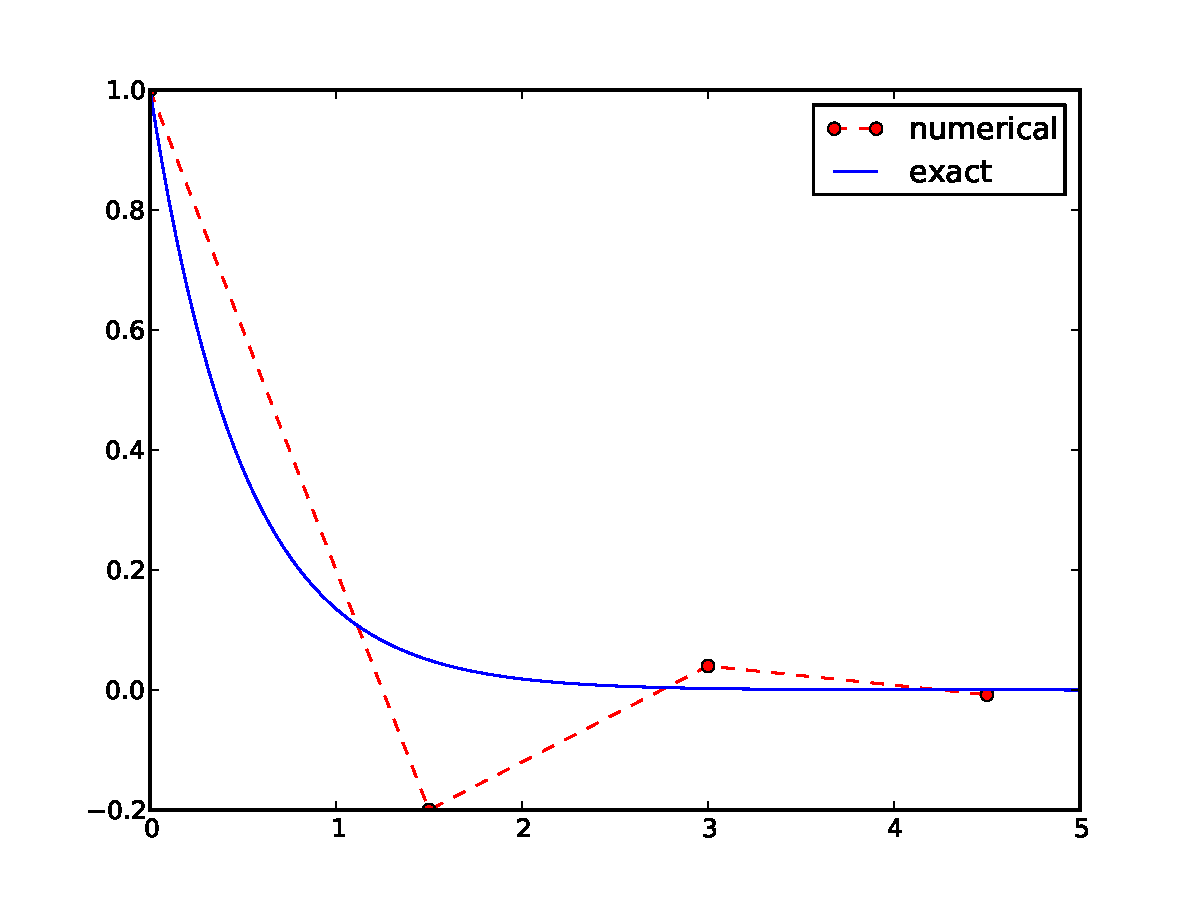
\includegraphics[width=0.4\linewidth]{../doc/slides/fig/CN_logo.pdf}}
}




\begin{frame}[plain,fragile]
\titlepage
\end{frame}

\begin{frame}[plain,fragile]
\frametitle{Goal}

The primary goal of this demo talk is to demonstrate how to write
talks with \href{{http://code.google.com/p/doconce}}{doconce}
and get them rendered in numerous HTML formats.

\begin{graybox1admon}[Layout.]
This version
utilizes beamer slides with the theme red3.
\end{graybox1admon}

\note{
The talk investigates the accuracy of three finite difference
schemes for the ordinary differential equation $u'=-au$ with the
aid of numerical experiments. Numerical artifacts are in particular
demonstrated.
}
\end{frame}

\begin{frame}[plain,fragile]
\frametitle{Mathematical problem}

\begin{columns}
\column{0.5\textwidth}
\begin{align}
u'(t) &= -au(t),
\label{ode}\\ 
u(0)  &= I,
\label{initial:value}
\end{align}

\begin{itemize}
 \item $t\in (0,T]$

 \item $a$, $I$, and $T$ are prescribed parameters

 \item $u(t)$ is the unknown function
\end{itemize}

\noindent

\column{0.5\textwidth}
\begin{center}  % inline figure
  \centerline{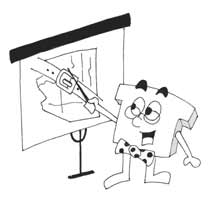
\includegraphics[width=0.5\linewidth]{../doc/slides/fig/teacher2.jpg}}
\end{center}


\end{columns}
\end{frame}

\begin{frame}[plain,fragile]
\frametitle{Numerical solution method}

\pause
\begin{block}{}
\begin{itemize}
 \item Mesh in time: $0= t_0< t_1 \cdots < t_N=T$

 \item Assume constant $\Delta t = t_{n}-t_{n-1}$

 \item $u^n$: numerical approx to the exact solution at $t_n$
\end{itemize}

\noindent
\end{block}



\pause
\begin{block}{}
Numerical scheme:
   \[
   u^{n+1} = \frac{1 - (1-\theta) a\Delta t}{1 + \theta a\Delta t}u^n,
   \quad n=0,1,\ldots,N-1
   \]
\end{block}
\end{frame}

\begin{frame}[plain,fragile]
\frametitle{Implementation}

The numerical method is implemented in a Python function:

\begin{minted}[fontsize=\fontsize{9pt}{9pt},linenos=false,mathescape,baselinestretch=1.0,fontfamily=tt,xleftmargin=7mm]{python}
def solver(I, a, T, dt, theta):
    """Solve u'=-a*u, u(0)=I, for t in (0,T] with steps of dt."""
    dt = float(dt)           # avoid integer division
    N = int(round(T/dt))     # no of time intervals
    T = N*dt                 # adjust T to fit time step dt
    u = zeros(N+1)           # array of u[n] values
    t = linspace(0, T, N+1)  # time mesh

    u[0] = I                 # assign initial condition
    for n in range(0, N):    # n=0,1,...,N-1
        u[n+1] = (1 - (1-theta)*a*dt)/(1 + theta*dt*a)*u[n]
    return u, t
\end{minted}
\end{frame}

\begin{frame}[plain,fragile]
\frametitle{The Crank-Nicolson method}

\begin{center}  % inline figure
  \centerline{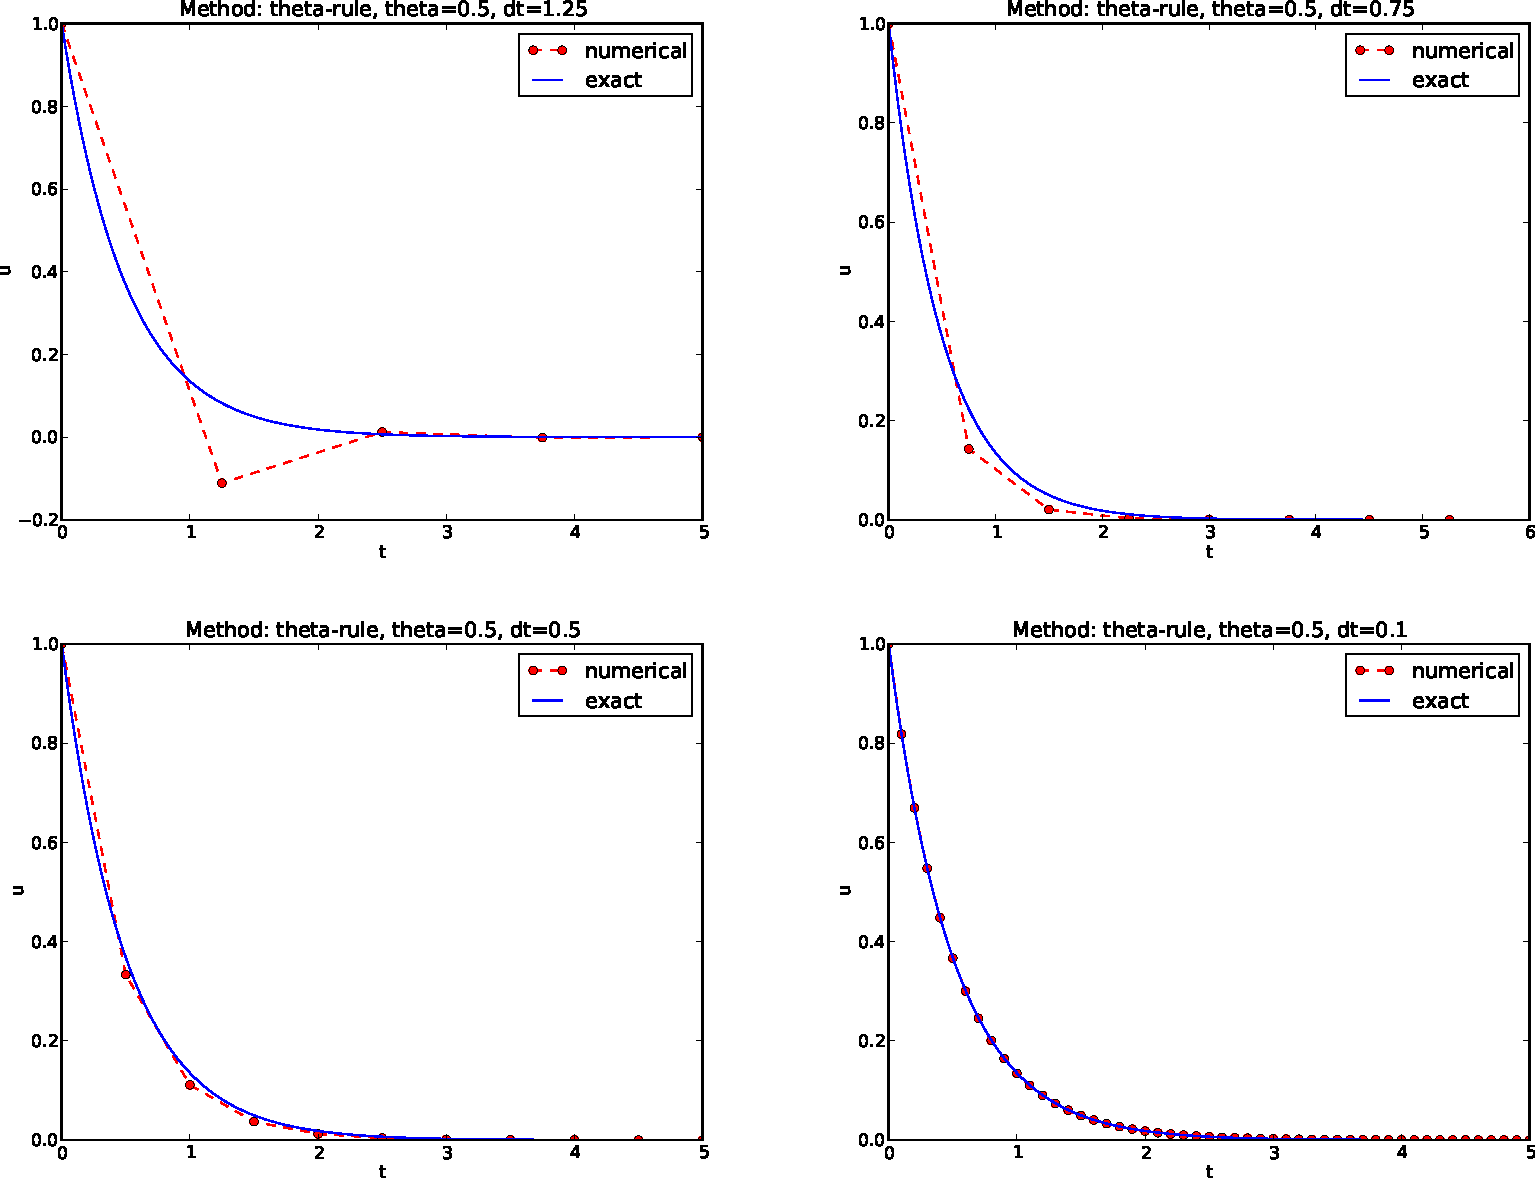
\includegraphics[width=0.9\linewidth]{../doc/slides/fig/CN.pdf}}
\end{center}
\end{frame}

\begin{frame}[plain,fragile]
\frametitle{The artifacts can be explained by some theory}

\pause
\begin{block}{}
Exact solution of the scheme:

\[ u^n = A^n,\quad A = \frac{1 - (1-\theta) a\Delta t}{1 + \theta a\Delta t}\thinspace .\]
\end{block}



\pause
\begin{block}{}
\begin{itemize}
 \item Stability: $|A| < 1$

 \item No oscillations: $A>0$

 \item Always for Backward Euler ($\theta=1$)

 \item $\Delta t < 1/a$ for Forward Euler ($\theta=0$)

 \item $\Delta t < 2/a$ for Crank-Nicolson ($\theta=1/2$)
\end{itemize}

\noindent
\end{block}



\pause
\begin{graybox1admon}[Concluding remarks:]
Only the Backward Euler scheme is guaranteed to always give
qualitatively correct results.
\end{graybox1admon}
\end{frame}

\end{document}
